\chapter{Methodology}
\label{chap:met}
\chaptermark{Methodology}

This chapter describes how the security work was carried out. It covers how the work was organised, which frameworks and standards were applied and how far, the threat model, and the tools used.

\section{Research Design}
\label{sec:met-design}

I planned the security work in seven steps: planning and requirements, choosing tools, design, building, testing before deployment, deployment, and checking afterwards. These were grouped under the functions of the NIST Cybersecurity Framework 2.0, and Figure \ref{fig:seven-phases} shows them. Five were completed at the time this was written; deployment, carried out by a teammate, had not fully succeeded, and the checks that follow deployment had not begun. Deployment has since been completed, every fix verified locally during this work is now live on the hospital's server, though the post-deployment checks (Section \ref{sec:conc-future}) remain outstanding. The five phases that ran did not run once each in order. Every time I checked something, I found a reason to change a decision I had already made, so the design, the build and the testing each came round more than once. That is why I call the method build-and-check cycles. The seven steps say what I planned; the cycles say how it actually ran.

\begin{figure}[H]
  \centering
  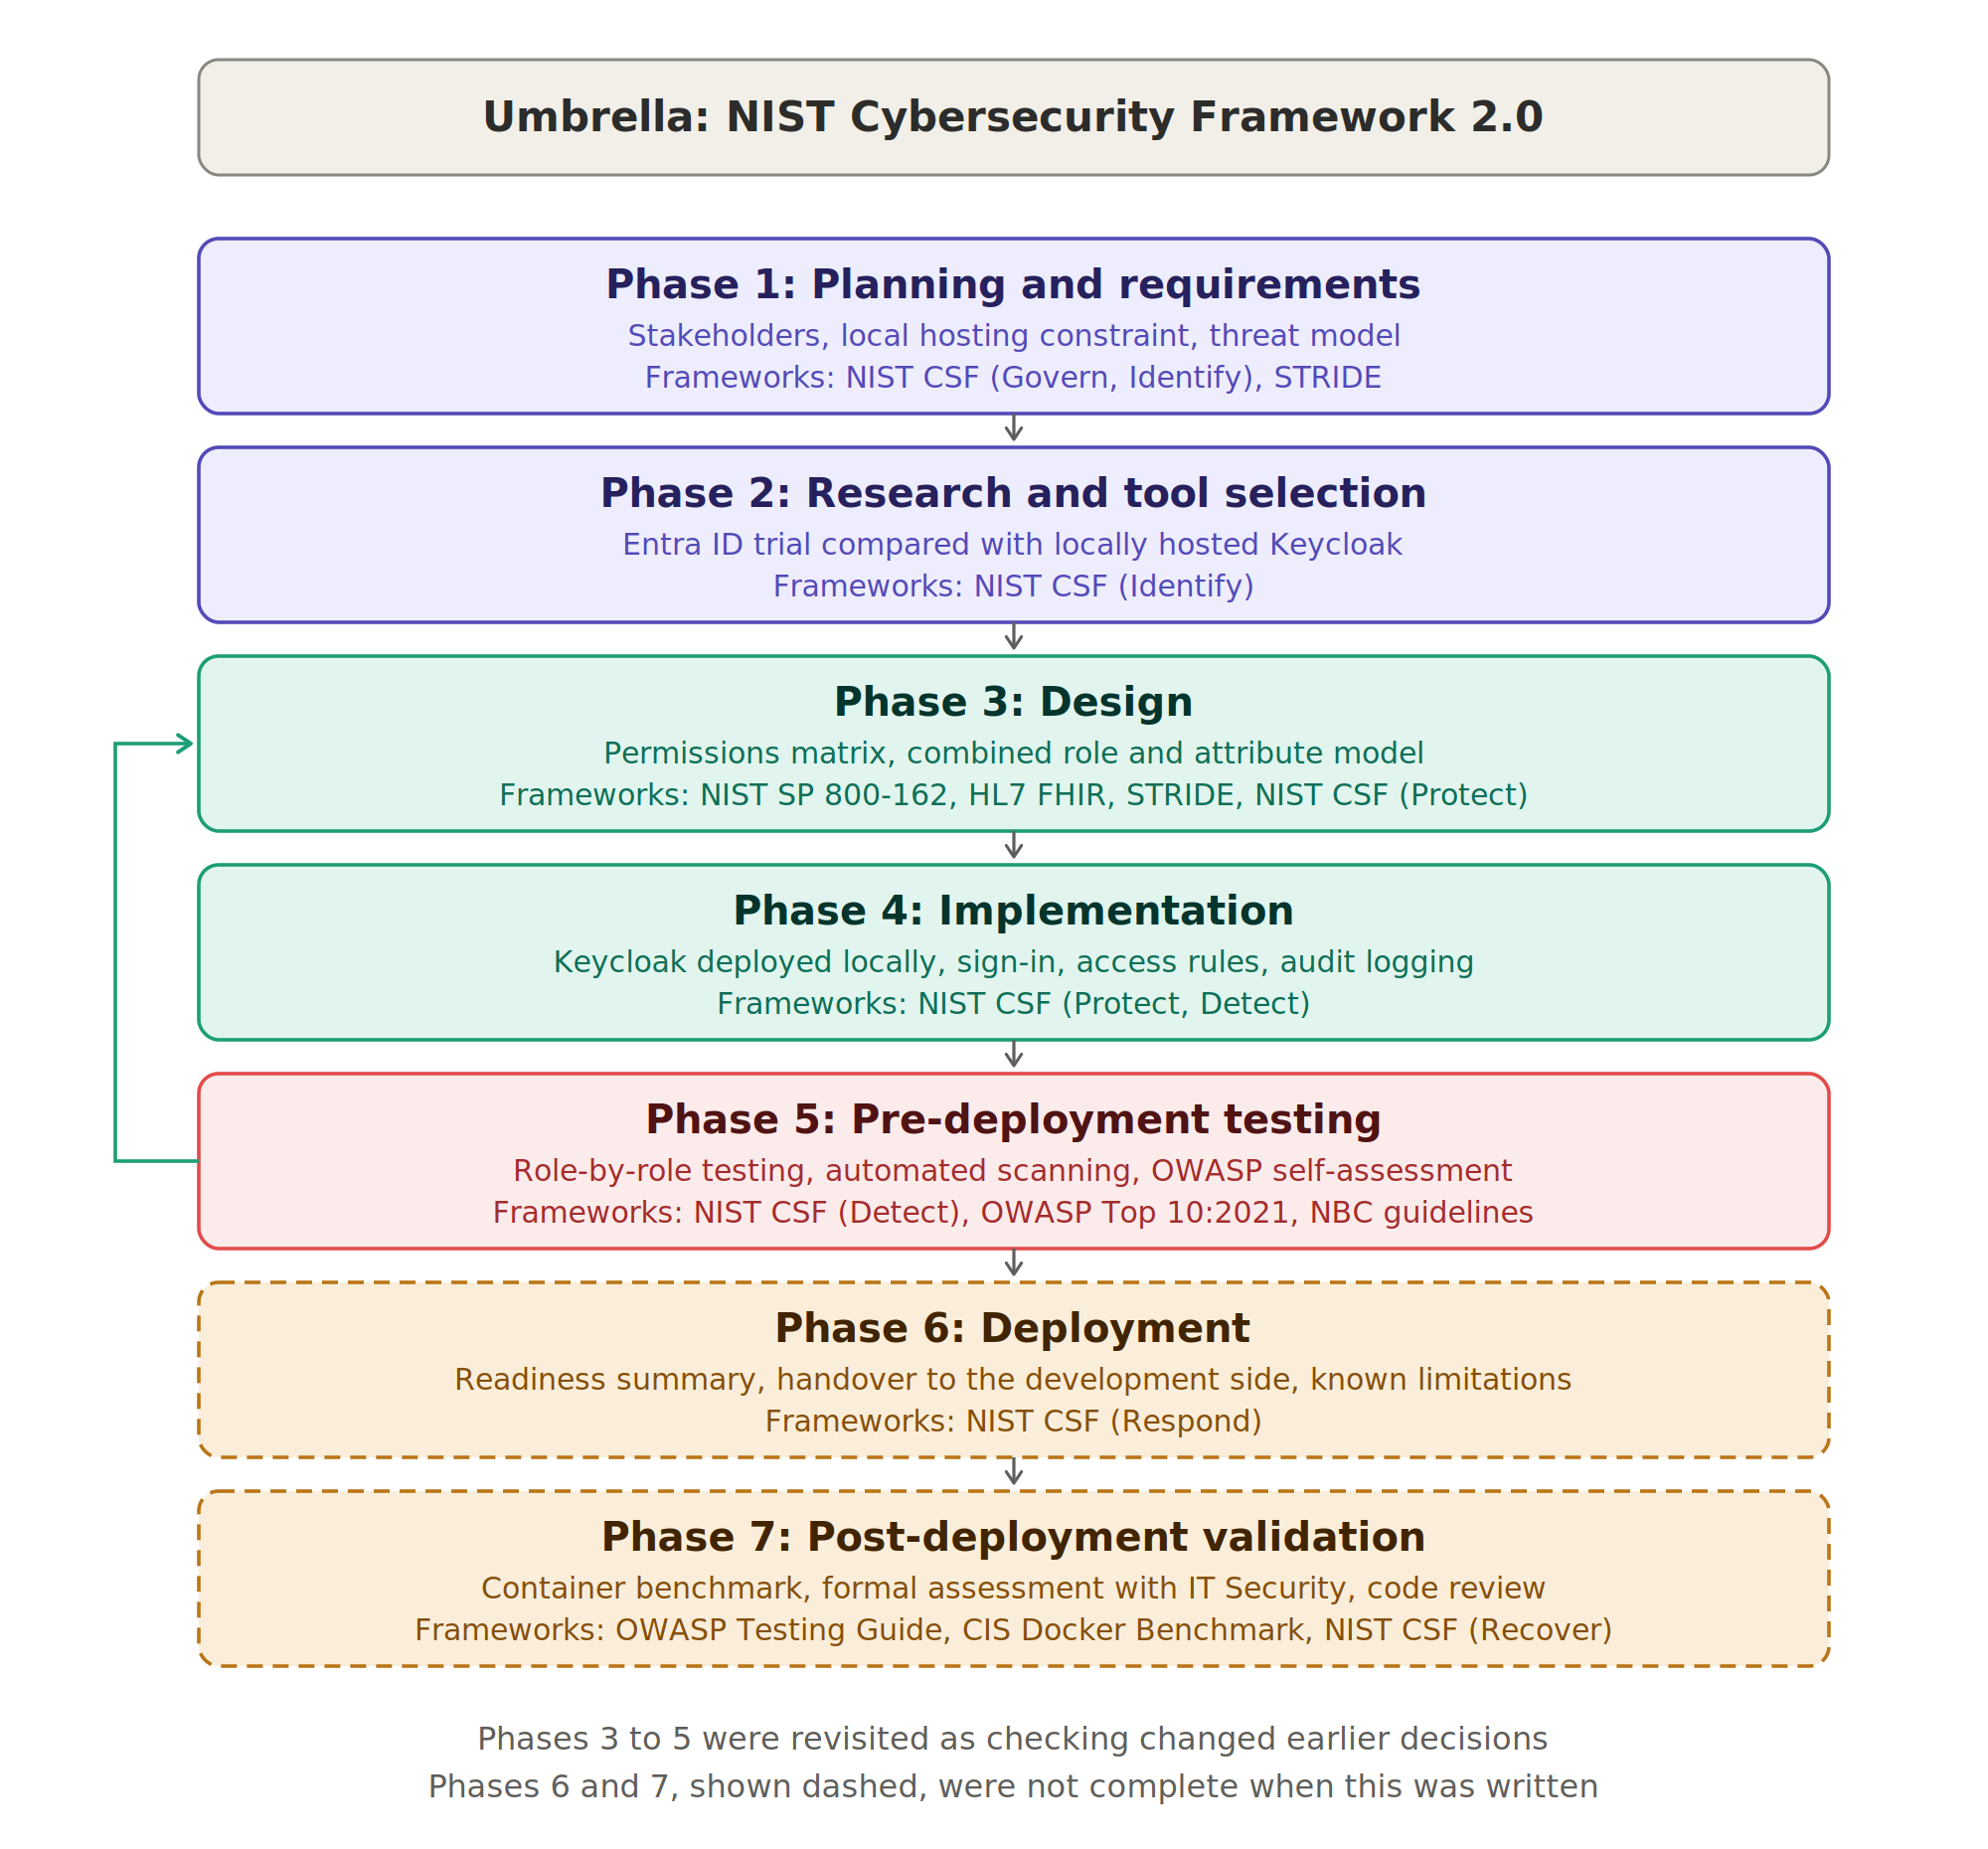
\includegraphics[width=\textwidth]{figs/Figure2-Seven-Phases.png}
  \caption{The seven phases of the security work, mapped to the functions of the NIST Cybersecurity Framework 2.0. Phases 3 to 5 were revisited as checking changed earlier decisions. Phases 6 and 7 were not complete at the time of writing.}
  \label{fig:seven-phases}
\end{figure}

The work covered four things: signing in, what each user may do, how their actions are recorded, and the security of the software the system runs on. Going round more than once mattered. I could not check the rules until I had written them, and I could not write them correctly until I had tested the system.

I did not begin from a written table. The code already existed, written by my teammate, so I started by reading it and writing down what it allowed each role to do. That gave the first version of the rules document. I then went through it against the workflow the team needed, adding rules and changing others, and writing down every difference I found. Some of those differences I could settle myself. Others needed the team to decide. A few are still open, because they depend on how staff want to work. Differences where the code was simply wrong were listed separately from differences where nobody had decided yet. Both lists are in the rules document. This review was the first of three checks.

The second check was manual testing, role by role, on the running system on my own machine. I signed in with one account for each of the five roles and followed a case from creation through to the insurer's decision. Where the system behaved differently from the rules, I recorded a finding. I then either fixed it, left it with a written reason, or closed it because the system was right and the rule was wrong.

The third check used automated tools on the same version of the code, in the same period: one for the packages the system depends on, one for the container images, one for passwords left in files, and one for the team's own code. I ran the scanners and the manual testing on the same version at the same time, on purpose. It means the two sets of findings can be compared directly, rather than across a version that had changed in between.

A fourth pattern ran alongside these three. I passed changes to the teammate handling deployment, and when a problem turned out to be on the security side, it was reported back to me, I corrected it, and passed it on again. Some problems only appeared once the system was installed, and those reached me through those reports rather than through my own testing.

Each cycle produced documents as well as code changes: the access control rules table, a record of each scan, an assessment against all ten OWASP categories, and a summary of what remained open and who owned it. I wrote these while working, not afterwards, and they are where the numbers in Chapter \ref{chap:result} come from.

I used AI tooling to help write and investigate code, under my direction. What to examine, whether a finding was real, and what to fix or defer were my decisions. I checked what the tooling reported against the running system before accepting it, and several reports turned out to be wrong.

\section{Frameworks and Standards Applied}
\label{sec:met-frameworks}

I applied frameworks selectively rather than in full. Table \ref{tab:frameworks} states which version I used and how far each one was applied, including the two that were planned but not carried out in this phase. Where a newer version has been published since this work was done, the version listed is the one that was current at the time, and re-assessment against the newer version is recorded in Section \ref{sec:conc-future}.

\begin{table}[H]
\centering
\caption{Frameworks and standards used, and how far each was applied.}
\label{tab:frameworks}
\begin{tabular}{|p{4cm}|p{2cm}|p{7.9cm}|}
\hline
\textbf{Framework} & \textbf{Version} & \textbf{Extent of application} \\
\hline
NIST Cybersecurity Framework & 2.0 (2024) & Six functions used to organise the work; control set not implemented \\
\hline
HL7 FHIR & R5 & Security section only \\
\hline
NIST SP 800-162 & 2014 & Definition and model of attribute-based access control \\
\hline
OWASP Top 10 & 2021 & All ten categories rated against evidence \\
\hline
NBC Technology and Cyber Risk Management Guidelines & 2026 & Access control, data security, audit trail and testing sections, used as a benchmark \\
\hline
OWASP ASVS & 4.0.3 (2021) & Level 2 target, all 14 chapters assessed, 62 subsections checked \\
\hline
STRIDE & --- & All six categories \\
\hline
CIS Docker Benchmark & --- & Not applied; planned for a later phase \\
\hline
OWASP Testing Guide & --- & Not applied; planned for a later phase \\
\hline
\end{tabular}
\end{table}

Each source did one job. The NIST Cybersecurity Framework gave the work its structure: the seven phases in Figure \ref{fig:seven-phases} follow its six functions \cite{nistcsf2}. The system's data model already follows FHIR, so FHIR's security section was the obvious place to look for decisions about signing in and encryption \cite{hl7fhir}. NIST SP 800-162 gave the access control model \cite{nist80162}. The OWASP Top 10 was the list I checked the code against \cite{owasp2021}. The National Bank of Cambodia's guidelines gave something to measure the result against, rather than a rule to comply with \cite{nbc2026}. The OWASP ASVS gave a second, more granular checklist: a separate pass at Level 2 across all fourteen chapters of the 4.0.3 edition, reported alongside the Top 10 results in Chapter \ref{chap:result} \cite{owaspasvs}. STRIDE gave the six categories used in the threat model described next \cite{stride}.

HIPAA and ISO/IEC 27001 were also considered. HIPAA was set aside because it is United States legislation, and this hospital is in Cambodia. ISO 27001, and its healthcare companion ISO 27799, require building a full organisation-wide information security management system. This includes ongoing risk registers, management review cycles, and certification audits. That scope was too large for a single feature built during a six-month placement. NIST CSF was used instead, selectively, as already described.

Two frameworks in the table were not used. The CIS Docker Benchmark checks how containers are set up and run. The OWASP Testing Guide sets out how to carry out a penetration test. Both belong to work that comes after deployment, neither had been done when this was written, and both are listed in Section \ref{sec:conc-future} as work that remains.

I only used parts of each framework, so I cannot say the system complies with any of them. What I can say is which specific requirements were met and which were not, and each one comes from a document I can point to. Read Chapter \ref{chap:result} that way, as findings measured against requirements, not as proof of compliance.

\section{Threat Modelling}
\label{sec:met-threat}

I used STRIDE: spoofing, tampering, repudiation, information disclosure, denial of service, and elevation of privilege, to sort the threats this system faces. I applied it after the system was built, not before. Its job was to file what testing had already found, and to check that no kind of threat had been missed. STRIDE gave the six categories. My findings filled them.

Five of the six hold defects found during this project. The sixth, denial of service, was not addressed, and is recorded as a limitation.

\begin{longtable}{|p{2.8cm}|p{4.3cm}|p{6.8cm}|}
\caption{STRIDE categories and the defects found in each.}
\label{tab:stride} \\
\hline
\textbf{Category} & \textbf{Threat in this system} & \textbf{What was found} \\
\hline
\endfirsthead
\multicolumn{3}{@{}l}{\textbf{Table \thetable} \ldots continued} \\
\hline
\textbf{Category} & \textbf{Threat in this system} & \textbf{What was found} \\
\hline
\endhead
\hline
\multicolumn{3}{r}{\textit{Continued on next page}} \\
\endfoot
\hline
\endlastfoot
Spoofing & Someone acts as a user they are not & A user belonging to no group received a valid session and could read every case. Signing out left the identity provider's session open, so the next person at a shared computer entered the previous user's account without a password. \\
\hline
Tampering & Case data changed by someone who should not be able to, or at a point when it should be locked & Doctors could alter the diagnosis and the cost after Finance had reviewed the case. Prices could be changed on cases already submitted or closed. A user could change their own display name, which relabelled every past audit entry for that person. \\
\hline
Repudiation & Someone denies an action, and the record cannot prove otherwise & When the system refused someone, it recorded nothing. Audit entries could not show which role had acted. A refused sign-in is recorded nowhere in the application, because sign-in stops before anything is written. Those attempts appear only in Keycloak's own log, so an investigation has to look in two places. The log stores a reference to the user, and looks up the name when the record is read. So a change of name changes every past entry for that person. \\
\hline
Information disclosure & Data reaches someone who should not see it & A surgeon's list included other surgeons' cases. Finance saw every case by dropping one URL parameter. Every role could read the full staff directory, including email addresses. Removing a patient identifier from the screen did not remove it from the data sent to the browser, where it can still be read. The connection is not encrypted, so patient data and session cookies cross the hospital network in readable form. \\
\hline
Denial of service & The system is knocked over so nobody can use it & Not addressed in this phase. \\
\hline
Elevation of privilege & A user gains rights they were not granted & Case creation was open to three roles instead of one. Submit and finalise sat with the wrong role. The page-level guard never ran at all. If creating a user's database record fails, the error is logged but the sign-in continues, so a session can exist with no record behind it. \\
\hline
\end{longtable}

Most of the findings are about people seeing what they should not, or doing what they should not. That is what you would expect from a system where five roles share the same cases. Both kinds are decided by the same three things: the user's role, whether the case is theirs, and how far the case has progressed.

Denial of service was not addressed in this phase. Being reachable only inside the hospital lowers the risk from an outside attacker. It does not remove the risk from a compromised or careless account inside the hospital. Testing for it was not reached in the time available. It is understood to be covered by Canadia Bank (IT security department)'s separate review, though those findings are confidential and not reproduced in this Graduation Project Report. It is recorded in Section \ref{sec:conc-future}.

\section{Tools and Technology}
\label{sec:met-tools}

The tools fall into two groups: those the system is built from, and those used to check it.

\begin{table}[H]
\centering
\caption{Tools used in the system and in its verification.}
\label{tab:tools}
\begin{tabular}{|p{6cm}|p{4.5cm}|p{3.4cm}|}
\hline
\textbf{Purpose} & \textbf{Tool} & \textbf{Version} \\
\hline
Identity provider & Keycloak & 26.7.2 \\
\hline
Application framework & Next.js & 15.5.24 \\
\hline
Session handling & Auth.js (NextAuth) & 5.0.0-beta.32 \\
\hline
Database & PostgreSQL & 16 \\
\hline
Database access and migrations & Prisma & 7.8.0 \\
\hline
FHIR server & HAPI FHIR & 7.4.0 \\
\hline
Hospital information system & ANZER, read-only & --- \\
\hline
Deployment & Docker / Docker Compose & 29.7.2 / v5.4.0 \\
\hline
Static analysis & Semgrep & --- \\
\hline
Container image scanning & Trivy & --- \\
\hline
Dependency scanning & npm audit & npm 11.12.1 \\
\hline
Secret scanning & secretlint & 13.0.2 \\
\hline
Browser-driven testing & Puppeteer & 25.3.0 \\
\hline
\end{tabular}
\end{table}

Semgrep and Trivy were run in July 2026. I did not fix which version of each tool was used, so both ran whatever release was current that day.

Keycloak was chosen after an extended trial of Microsoft Entra ID. The hospital needed the system to run on hospital-owned servers, and Entra ID runs only as a cloud service. Keycloak also supports user federation with the hospital's own Active Directory, so staff sign in with the same credentials they already use elsewhere in the hospital, rather than remembering a separate username and password for this system. The application itself never stores or handles user passwords, since sign-in is delegated to Keycloak and, through it, to the hospital's AD. This also matched FHIR's security guidance, which recommends OAuth \cite{hl7fhir}, so the choice fit both the hospital's requirements and the standard the data model follows. Auth.js keeps a user logged in, and the version used is a beta; the makers have not marked it finished, though many production systems use it.

CodeQL and Semgrep both read code looking for mistakes; CodeQL is free only for public code and this project is private, so I used Semgrep, which runs on my own machine.

Each kind of data lives in a different place. Roles are held in Keycloak; the application reads them from the token. Patient records come from ANZER, which this project reads but does not own, change, or assess. Case data and the audit trail sit in the application's own PostgreSQL database. The FHIR server is bound to the local interface, so no other machine can reach it.
